% *********************************************************************
% © 2021–2026 Jeremy Sylvestre
%
% Permission is granted to copy, distribute and/or modify this document
% under the terms of the GNU Free Documentation License, Version 1.3 or
% any later version published by the Free Software Foundation; with no
% Invariant Sections, no Front-Cover Texts, and no Back-Cover Texts. A
% copy of the license is included in the appendix entitled “GNU Free
% Documentation License” that appears in the output document of this
% PreTeXt source code. All trademarks™ are the registered® marks of
% their respective owners.
%
% *********************************************************************

\newcommand*{\xmin}{-0.075}
\newcommand*{\xmax}{1.1}
\newcommand*{\ymin}{-0.25}
\newcommand*{\ymax}{1.25}

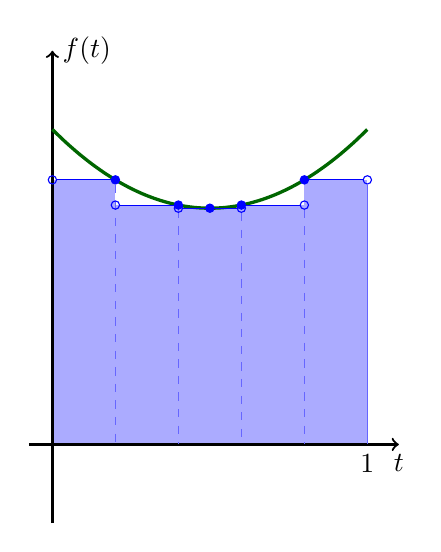
\begin{tikzpicture}
[
	closedpt/.style={circle,draw,fill,inner sep=0pt,minimum size=3pt},
	openpt/.style={circle,draw,inner sep=0pt,minimum size=3pt},
	scale=4
]

	% rectangle fills
	\fill[blue, opacity=0.33] (0,0.84) rectangle (0.2,0);
	\fill[blue, opacity=0.33] (0.2,0.76) rectangle (0.4,0);
	\fill[blue, opacity=0.33] (0.4,0.75) rectangle (0.6,0);
	\fill[blue, opacity=0.33] (0.6,0.76) rectangle (0.8,0);
	\fill[blue, opacity=0.33] (0.8,0.84) rectangle (1,0);

	% label horiz axis
	\node[below] at (1,0) {$1$};

	% axes
	\draw[->,thick] (\xmin,0) -- (\xmax,0) node[below] {$t$};
	\draw[->,thick] (0,\ymin) -- (0,\ymax) node[right] {$f(t)$};

	% continuous graph
	\draw[green!40!black,very thick,domain=0:1,smooth] plot (\x,{\x^2 - \x + 1});

	% levels and dividers
	\node[blue,openpt] at (0,0.84) (start) {};
	\node[blue,closedpt] at (0.2,0.84) (stop) {};
	\draw[blue,thin] (start.east) -- (stop.west);
	\draw[blue!60!white,dashed] (stop.south) -- (0.2,0);
	%
	\node[blue,openpt] at (0.2,0.76) (start) {};
	\node[blue,closedpt] at (0.4,0.76) (stop) {};
	\draw[blue,thin] (start.east) -- (stop.west);
	\draw[blue!60!white,dashed] (stop.south) -- (0.4,0);
	%
	\node[blue,openpt] at (0.4,0.75) (start) {};
	\node[blue,closedpt] at (0.5,0.75) {};
	\node[blue,openpt] at (0.6,0.75) (stop) {};
	\draw[blue,thin] (start.east) -- (stop.west);
	\draw[blue!60!white,dashed] (stop.south) -- (0.6,0);
	%
	\node[blue,closedpt] at (0.6,0.76) (start) {};
	\node[blue,openpt] at (0.8,0.76) (stop) {};
	\draw[blue,thin] (start.east) -- (stop.west);
	\draw[blue!60!white,dashed] (stop.south) -- (0.8,0);
	%
	\node[blue,closedpt] at (0.8,0.84) (start) {};
	\node[blue,openpt] at (1,0.84) (stop) {};
	\draw[blue,thin] (start.east) -- (stop.west);
	\draw[blue!60!white] (stop.south) -- (1,0);


\end{tikzpicture}
